% Document setup
\documentclass[12pt]{article}
\usepackage[margin=1in]{geometry}
\usepackage{fancyhdr}
\usepackage{lastpage}

\pagestyle{fancy}
\lhead{Richard Whitehill}
\chead{PHYS 804 -- HW \HWnum}
\rhead{\duedate}
\cfoot{\thepage \hspace{1pt} of \pageref{LastPage}}

% Encoding
\usepackage[utf8]{inputenc}
\usepackage[T1]{fontenc}

% Math/Physics Packages
\usepackage{amsmath}
\usepackage{amssymb}
\usepackage{mathtools}
\usepackage{physics}
\usepackage{siunitx}

\AtBeginDocument{\RenewCommandCopy\qty\SI}

% Enumeration/itemize
\usepackage{enumitem}
\newenvironment{parts}
{\begin{enumerate}[label=\textbf{(\alph*)},leftmargin=*,itemsep=-10pt]
}{\end{enumerate}}

% Reference Style
\usepackage{hyperref}
\hypersetup{
    colorlinks=true,
    linkcolor=blue,
    filecolor=magenta,
    urlcolor=cyan,
    citecolor=green
}

\newcommand{\eref}[1]{Eq.~(\ref{eq:#1})}
\newcommand{\erefs}[2]{Eqs.~(\ref{eq:#1})--(\ref{eq:#2})}

\newcommand{\fref}[1]{Fig.~\ref{fig:#1}}
\newcommand{\frefs}[2]{Figs.~\ref{fig:#1}--\ref{fig:#2}}

\newcommand{\tref}[1]{Table~\ref{tab:#1}}
\newcommand{\trefs}[2]{Tables~\ref{tab:#1}-\ref{tab:#2}}

% Figures and Tables 
\usepackage{graphicx}
\usepackage{float}
\usepackage[font=small,labelfont=bf]{caption}

\newcommand{\bef}{\begin{figure}[h!]\begin{center}}
\newcommand{\eef}{\end{center}\end{figure}}

\newcommand{\bet}{\begin{table}[h!]\begin{center}}
\newcommand{\eet}{\end{center}\end{table}}

% tikz
\usepackage{tikz}
\usetikzlibrary{calc}
\usetikzlibrary{decorations.pathmorphing}
\usetikzlibrary{decorations.markings}
\usetikzlibrary{arrows.meta}
\usetikzlibrary{positioning}
\usetikzlibrary{3d}
\usetikzlibrary{shapes.geometric}

% tcolorbox
\usepackage[most]{tcolorbox}
\usepackage{xcolor}
\usepackage{xifthen}
\usepackage{parskip}

\newcommand*{\eqbox}{\tcboxmath[
    enhanced,
    colback=black!10!white,
    colframe=black,
    sharp corners,
    size=fbox,
    boxsep=8pt,
    boxrule=1pt
]}

% problem-solution macros
% \usepackage{adjustbox}
\usepackage{changepage}

\newtcolorbox{probbox}[1][]{
    breakable,
    enhanced,
    boxrule=0pt,
    frame hidden,
    borderline west={4pt}{0pt}{green!50!black},
    colback=green!5,
    before upper=\textbf{Problem #1) \,},
    % \textbf{Problem #1 \ifthenelse{\isempty{#1}}{}{: #1} \\ },
    sharp corners,
    parbox=false
}

% \newtcolorbox{ProblemBox}[1][]{%
%   breakable,
%   enhanced,
%   colback=black!10!white,
%   colframe=black,
%   title={\large #1 \hfill}
% }
\newcommand{\prob}[2]{
\begin{probbox}[#1]
#2
\end{probbox}
}

\newenvironment{solution}{\begin{adjustwidth}{8pt}{8pt}}{\end{adjustwidth}}
\newcommand{\sol}[1]{
\begin{solution}
#1
\end{solution}
}
% \textbf{#1)} #2}

% Miscellaneous Definitions/Settings
\newcommand{\reals}{\mathbb{R}}
\newcommand{\integers}{\mathbb{Z}}
\newcommand{\naturals}{\mathbb{N}}
\newcommand{\rationals}{\mathbb{Q}}
\newcommand{\complexs}{\mathbb{C}}

\setlength{\parskip}{\baselineskip}
\setlength{\parindent}{0pt}
\setlength{\headheight}{14.49998pt}
\addtolength{\topmargin}{-2.49998pt}


\def\HWnum{Final Project}
\def\duedate{December 9, 2024}


\begin{document}

\section{Introduction}
\label{sec:introduction}

In a previous project this semester we have solved the time-independent Schr\"{o}dinger equation or energy eigenvalue equation by transforming it from a continuous second-order differential equation in space to a dicscrete eigenvalue problem.
For this problem, though, we were only interested in obtaining bound state solutions and entirely neglected the scattering states.
Since the time of Rutherford, results from scattering theory and experiments have provided us essential information about the structure and contents of our universe, and therefore, these scattering states are important in their own right.

For this work, we would like to explore scattering numerically in one dimension.
Even though from the outset this seems quite restrictive, developing the scattering formalism in one dimension will be quite instructive, and in addition, many three dimensional problems, namely those related to central potentials, can be reduced to one dimensional problems.

\section{Mathematical framework}
\label{sec:mathematical-framework}


The time-independent Schr\"{o}dinger equation is given by\footnote{Note that we work in natural units where $\hbar = c = 1$.}
\begin{align}
    -\frac{1}{2m} \dv[2]{\psi_{E}(x)}{x} + V(x) \psi_{E}(x) = E \psi_{E}(x)
,\end{align}
where $E$ is the energy eigenvalue of this equation and $\psi_{E}(x)$ is the corresponding eigenfunction.
When $E < \lim_{|x| \rightarrow \infty} V(x)$, we have bound states, usually discrete levels, which are normalizable since they fall off exponentially as $|x| \rightarrow \infty$.
On the other hand, when $E$ is larger than the potential in one of these asymptotic regions, we have a scattering state, and have a continuum of solutions.
In the asymptotic regions, however, our solutions are of the generic form $e^{\pm i k x}$ and are therefore not normalizable and hence not physical.
To solve definite problems, we must work with physical solutions in the context of wavepackets of the form
\begin{align}
    \psi(x) = \int \frac{\dd{k}}{\sqrt{2 \pi}} \widetilde{\psi}(k) e^{i k x}
,\end{align}
where the time-dependence can be generated by the time-evolution operator.
Taking motivation from this, we simulate scattering, which inherently requires dynamics, in two ways. 

\subsection{Finite differences}
\label{ssec:finite-differences}

For our first numerical method, we solve the time-dependent Schr\"{o}dinger equation 
\begin{align}
    i \pdv{\Psi(x,t)}{t} = -\frac{1}{2m} \pdv[2]{\Psi(x,t)}{x} + V(x) \Psi(x,t)
.\end{align}
directly by implementing a finite difference scheme.
Using a forward difference formula for the time derivative, the three-point formula for the second derivative, and rearranging, we obtain
\begin{align}
    \Psi_{n}^{(m + 1)} = \Psi_{n}^{(m)} + i \Delta t \Bigg( \frac{\Psi_{n-1}^{(m)} - 2 \Psi_{n}^{(m)} + \Psi_{n+1}^{(m)}}{2m \Delta x^2} - V_{n} \Psi_{n}^{(m)} \Bigg)
,\end{align}
where $\Psi_{n}^{(m)} = \Psi(x_n,t_{m})$, $x_{n} = x_0 + n \Delta x$, and $t_{m} = m \Delta t$.
Thus, we have a sequence defined by $\Psi_{n}^{(m)} = U^{m} \Psi_{n}^{(0)}$, where
\begin{align}
    U_{kn} = \delta_{kn} - i \Delta t H_{kn}
,\end{align}
where the discretized Hamiltonian
\begin{align}
    H_{kn} = -\frac{\delta_{k-1,n} - 2 \delta_{kn} + \delta_{k+1,n}}{2m \Delta x^2} + V_{k} \delta_{kn}
.\end{align}
Such an equation reminds us of the unitary time evolution, which can be explored by direct matrix multiplication:
\begin{align}
    U_{kn}^{\dagger} U_{nk'} &= ( \delta_{kn} + i \Delta t H_{kn}^{\dagger} ) ( \delta_{nk'} - i \Delta t H_{nk'} ) = \delta_{k k'} + i \Delta t ( H_{kk'}^{\dagger} - H_{kk'} ) + \Delta t^2 H_{kn}^{\dagger} H_{nk'} \nonumber \\
    &= \delta_{kk'} + \mathcal{O}(\Delta t^2)
.\end{align}
Herein lies a primary difficulty of implementing this method: the eigenvalues of $U$ essentially scale the eigenvector components of our initial wavevector.
Hence, for stability, we would like to select $\Delta t$ and $\Delta x$ such that all of these eigenvalues are less than one.
Unfortunately, this is not possible since the eigenvalues of a unitary matrix have unit norm, prohibiting us from performing our time evolution in this manner.

{\color{red} 
    Move this section to the appendix.

    Make plots demonstrating instability.
}


\subsection{Fourier transform}
\label{ssec:fourier-transform}

If we cannot perform time evolution directly, perhaps we can take inspiration from a different place.
We know from quantum mechanics that our unitary time evolution operator $U(t,t')$ acts as $\Psi(x,t) = U(t,t') \Psi(x,t')$ and therefore satisfies the differential equation
\begin{align}
    i \pdv{U(t,t')}{t} = H U(t,t')
,\end{align}
which has solution
\begin{align}
    U(t,t') = e^{-i H (t - t')}
\end{align}
if $H$ is independent of time, which will be the case in our scattering problems.
Let us write $H = H_0 + V$, where $H_0$ is the free-particle Hamiltonian and $V$ contains the potential terms.
If we select our time step $\Delta t$ between time slices $t_{m}$ and $t_{m+1}$, then using the Baker-Campbell-Hausdorff formula, we can write
\begin{align}
    U(\Delta t) = e^{-i H \Delta t} \approx e^{-i H_0 \Delta t} e^{-i V \Delta t} \Big( 1 + \mathcal{O}(\Delta t^2) \Big)
.\end{align}
Since we are working in the context of wave-packets, we can act directly on the state at time $t_{m}$ as follows
\begin{align}
    \Psi(x,t_{m+1}) &= U(\Delta t) \Psi(x,t_{m}) = e^{-i V(x) \Delta t} \int \frac{\dd{k}}{\sqrt{2 \pi}} \widetilde{\Psi}(k,t_{m}) e^{-i H_0 \Delta t} e^{i k x} \nonumber \\
    &= e^{-i V(x) \Delta t} \int \frac{\dd{k}}{\sqrt{2 \pi}} \widetilde{\Psi}(k,t_{m}) e^{- i k^2 \Delta t / (2m)} e^{i k x}
.\end{align}
Thus, for small time steps, our potential changes the phase of the wave-function locally and the free part of the Hamiltonian propagates our modes according to their velocity $k/m$.

Because the above equation is set up on the continuous spatial domain we could set up our wave-packets as functions numerically and implement a numerical quadrature to take the Fourier transform at each $x$, but this could become quite computationally expensive, resource and time-wise.
Another approach utilizes the fast-fourier transform, which requires us to discretize our spatial domain.
Doing so, however, also requires the conjugate momentum domain to be discretized.
The details for computing the Fourier transform above can be found in App. \ref{app:relating-the-continuous-and-discrete-fourier-transforms}.

One thing to note with this method is that we have not imposed boundary conditions explicitly, but it can be seen that the Fourier method implicitly imposes periodic boundary conditions such that $\psi(x + L) = \psi(x)$.
That is, any part of the wave packet which physically exits our numerically imposed spatial region to the right appears back on the left part of our spatial domain.
It will befall us then to deal with such a non-physical behavior by either simulating our scattering events on a grid much larger than the extent of our potential or imposing some extra non-physical layers which damp the waves in order to minimize their effect when they exit the numerical domain and reappear.


\section{Freely propagating Gaussian wave packet}
\label{sec:freely-propagating-gaussian-wave-packet}

To test that our numerical solver works, we choose an initial wave function
\begin{align}
    \Psi(x,0) = \frac{1}{(2 \pi \sigma^2)^{1/4}} \exp{-\frac{(x - x_{0})^2}{4 \sigma^2}} \exp{i k x}
,\end{align}
which is a Gaussian density at $t = 0$ with average momentum $k$.
We can now use propagator formalism to determine the wave function at any later time $t$ as follows:
\begin{align}
\label{eq:gauss-wave-prop}
    \Psi(x,t) &= \int \dd{x'} K(x,x';t) \Psi(x',0) \nonumber \\
              &= \sqrt{\frac{m}{2 \pi i t}} \frac{1}{(2 \pi \sigma^2)^{1/4}} \int_{-\infty}^{\infty} \dd{x'} \exp{-\frac{m(x - x')^2}{2 i t} - \frac{(x' - x_0)^2}{4 \sigma^2} + i k x'}
.\end{align}
The intermediate form of the wave function is not too interesting for our purposes, but the probability density
\begin{align}
    |\Psi(x,t)|^2 = \frac{1}{\sqrt{2 \pi \sigma^2}} \frac{2 \sigma^2 m}{\sqrt{ 4 \sigma^4 m^2 + t^2 }} \exp{ -\frac{2 m^2 \sigma^2 [ x - (x_0 + k t / m) ]^2}{4 \sigma^{4} m^2 + t^2} }
.\end{align}


\begin{figure}[tb]
    \centering
    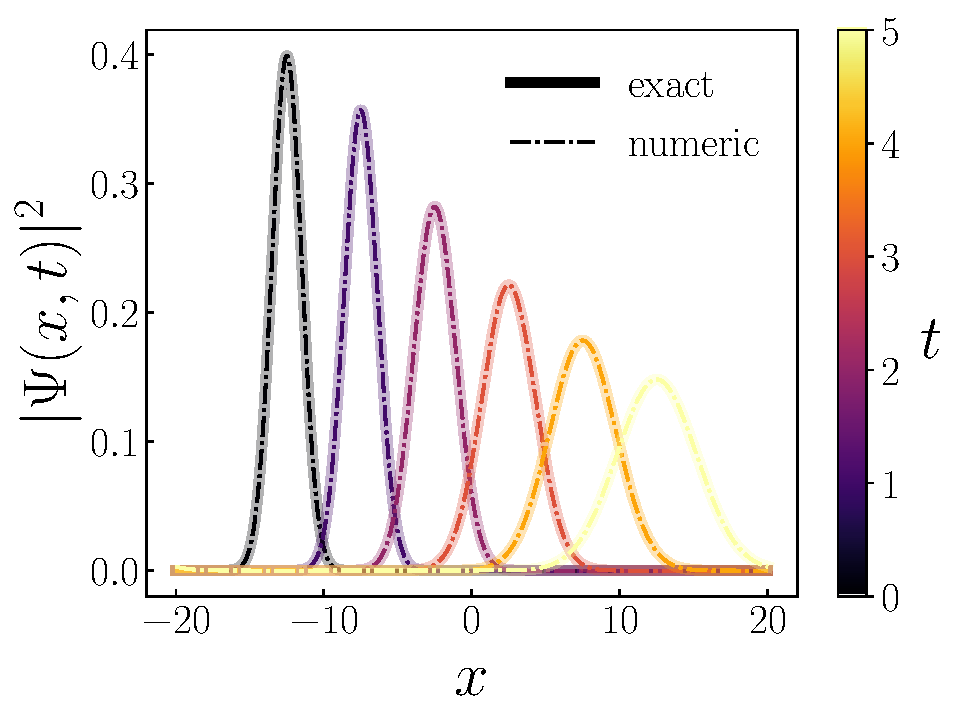
\includegraphics[width=0.7\linewidth]{gauss_wave-prop.pdf}
    \caption{Comparison of Gaussian wave-packet propagation, where the exact formula is given in Eq. \ref{eq:gauss-wave-prop}, with the numerical Fourier transform based numerical scheme presented in Sec. \ref{ssec:fourier-transform}.}
    \label{fig:gauss-wave-prop}
\end{figure}


\section{Wave packet treatment}
\label{sec:wave-packet-treatment}

We would like to understand the behavior of a single particle in the presence of a potential, in one-dimension for the sake of simplicity for now.
As always, at its core, this problem requires us to solve the Schr\"{o}dinger equation
\begin{align}
    i \pdv{\Psi(x,t)}{t} = H \Psi(x,t)
.\end{align}
Of course, this is done with the time evolution operator introduced already such that $\Psi(x,t) = e^{-i H t} \Psi(x,0)$.
Working in the context of wave packets, our potentials must be localized such that in the asymptotic regions $|x| \rightarrow \infty$ and the wave packet set up at $t = 0$ as
\begin{align}
    \Psi(x,0) = \int \frac{\dd{k}}{\sqrt{2 \pi}} \widetilde{\Psi}(k) e^{i k x}
\end{align}
is exactly the expansion of free particle eigenstates far from the potential.
Then, the time-evolution follows as
\begin{align}
    \Psi(x,t) = \int \frac{\dd{k}}{\sqrt{2 \pi}} \widetilde{\Psi}(k) e^{i k x - k^2 t / 2m}
.\end{align}
Thus, to analyze scattering problems, we can solve the time-independent energy eigenvalue equation for a given $k$ in the continuum of scattering states, determine the relative amplitudes of the incoming and outgoing pieces, and finally use this to determine the behavior of the system for $t \rightarrow \infty$ when our particles are far from the potential and are essentially free particles.


\subsection{Example: Scattering from a Dirac-$\delta$ source}

The example of an infinite pulse centered at $x = 0$ as $V(x) = V_0 \delta(x)$ is a fairly simple example to understand the analytic treatment of scattering in one dimension.
Because we send particles from left to right (i.e. $k > 0$), we choose the energy eigenstate corresponding to momentum $k > 0$ as
\begin{align}
    \psi_{k}(x) = 
    \begin{cases}
        e^{i k x} + A e^{-i k x} & x < 0 \\
        B e^{i k x} & x > 0
    .\end{cases}
\end{align}
For our boundary conditions, we have $\psi_{k}(0^{-}) = \psi_{k}(0^{+})$ and $\psi_{k}'(0^{+}) - \psi_{k}'(0^{-}) = 2 m V_0 \psi_{k}'(0)$.
Solving, we find
\begin{align}
    A &= -\frac{i V_0 m}{k + i V_0 m} \\
    B &= \frac{k}{k + i V_0 m}
.\end{align}
We can then construct a wave-packet for all times $t$ by summing these energy eigenstates as follows:
\begin{align}
    \Psi(x,t) &= \int \frac{\dd{k}}{\sqrt{2 \pi}} g(k) \psi_{k}(x) \nonumber \\
              &= \Theta(-x) \Bigg\{ \int_{0}^{\infty} \frac{\dd{k}}{\sqrt{2 \pi}} g(k) e^{i k x - i k^2 t / (2m)} + \int_{0}^{\infty} \frac{\dd{k}}{\sqrt{2 \pi}} g(k) A(k) e^{-i k x - i k^2 t / (2m)} \Bigg\} \nonumber \\
              &+ \Theta(x) \int_{0}^{\infty} \frac{\dd{k}}{\sqrt{2 \pi}} g(k) B(k) e^{i k x - i k^2 t / (2m)}
,\end{align}
where $g(k)$ is some properly chosen real profile function.
The analysis is made more tractable and cleaner if our wave packets have momentum modes sharply centered at some $k = k_0$.
Making this assumption, we proceed via the method of stationary phase.
Let us analyze the form of each term separately, beginning with the incident wave packet
\begin{align}
    \Psi_{I}(x,t) = \int_{0}^{\infty} \frac{\dd{k}}{\sqrt{2 \pi}} g(k) e^{i \varphi_{I}(x,t,k)}
,\end{align}
where $\varphi_{I}(x,t,k) = kx - k^2 t / 2m$.
Since $g(k)$ is sharply peaked around some $k_0$, we expand the phase function about $k_{0}$ as
\begin{align}
    \varphi_{I}(x,t,k) &= \varphi_{I}(x,t,k_0) + (k - k_0) \dv{\varphi_{I}}{x}\Big|_{k=k_0} + \mathcal{O}\Big( (k - k_0)^2 \Big) \nonumber \\
                       &= \varphi_{I}(x,t,k_0) + (k - k_0) (x - x_{i}(t)) + \mathcal{O}\Big( (k - k_0)^2 \Big)
,\end{align}
where $x_{I}(t) = k_0 t / m$ satisfies $\dv*{\varphi_{I}}{k}|_{k=k_0,x=x_{I}(t)}$ and is representative of the center of our incoming wave packet.
Using this, 
\begin{align}
    \Psi_{I}(x,t) \approx e^{i \varphi_{I}(x,t,k_{0})} \int_{0}^{\infty} \frac{\dd{k}}{\sqrt{2 \pi}} g(k) e^{i (k - k_0) (x - x_{I}(t))}
.\end{align}
Observe also that since $k$ is sharply peaked around $k = k_0 > 0$, it is inconsequential to extend the integration range to all $k$ as
\begin{align}
    \Psi_{I}(x,t) &\approx e^{i \varphi_{I}(x,t,k_0)} \int \frac{\dd{k}}{\sqrt{2 \pi}} g(k) e^{i (k - k_0) (x - x_{I}(t))} = e^{i [ \varphi_{I}(x,t,k_0) - k_0 (x - x_{I}(t)) ]} \int \frac{\dd{k}}{\sqrt{2 \pi}} g(k) e^{i k ( x - x_{I}(t) )} \nonumber \\
                  &= e^{i[\varphi_{I}(x,t,k_0) - k_0 (x - x_{I}(t))]} G(x - x_{I}(t),0)
,\end{align}
where $G(x)$ is the inverse Fourier transform of $g(k)$.

Next, we analyze the form of the reflected wave packet.
Defining
\begin{align}
    \Psi_{R}(x,t) = \int_{0}^{\infty} \frac{\dd{k}}{\sqrt{2 \pi}} g(k) |A(k)| e^{-i \chi_{A}(k)} e^{-i k x - i k^2 t / (2m)}
,\end{align}
so that overall reflected phase function
\begin{align}
    \varphi_{R}(x,t,k) = kx + \frac{k^2 t}{2m} + \chi_{A}(k)
\end{align}
with
\begin{align}
    \tan{\chi_{A}(k)} = - \frac{\Im{A(k)}}{\Re{A(k)}} = -\frac{k}{m V_0}
.\end{align}
Performing the stationary phase expansion, we find
\begin{align}
    \varphi_{R}(x,t,k) \approx \varphi_{R}(x,t,k_0) + (k - k_0) (x - x_{R}(t))
,\end{align}
where 
\begin{align}
    x_{R}(t) &= - \frac{k_0 t}{m} - \chi_{r}'(k_0) = -\frac{k_0 t}{m} + \frac{1}{m V_0} \frac{1}{1 + {\rm arctan}^2(k_0 / m V_0)} \nonumber \\
    &= -\frac{k_0}{m} \Bigg\{ t - \frac{1}{k_0 V_0} \frac{1}{1 + \arctan^2(k_0/m V_0)} \Bigg\}
.\end{align}
With this, we have
\begin{align}
    \Psi_{R}(x,t) = |A(k_0)| e^{i [ \varphi_{R}(x,t,k_0) - k_0(x - x_{R}(t)) ]} G(x - x_{R}(t))
.\end{align}
Similarly, for the transmitted wave packet
\begin{align}
    \Psi_{T}(x,t) &= \int_{0}^{\infty} \frac{\dd{k}}{\sqrt{2 \pi}} g(k) |B(k)| e^{i \varphi_{T}(x,t,k)} \\
    \varphi_{T}(x,t,k) &= k x - k^2 t / (2m) - \chi_{B}(k)
,\end{align}
so that
\begin{align}
    x_{T}(t) = \frac{k_0 t}{m} + \chi_{B}'(k) = \frac{k_0}{m} \Bigg\{ t - \frac{m^2 V_0}{k_0^3} \frac{1}{1 + \arctan^2(m V_0 / k_0)} \Bigg\}
\end{align}
and
\begin{align}
    \Psi_{T}(x,t) = |B(k_0)| e^{i [ \varphi_{T}(x,t,k_0) - k_0 ( x - x_{T}(t) ) ]} G(x - x_{T}(t))
.\end{align}

The upshot of all this work is the following.
When we prepare a wave packet with a very narrow momentum spectrum that is sent towards a localized momentum, then after a sufficient amount of time (determined by the particle's mass and average momentum as well as the specifics of the potential) we observe reflected and transmitted wave packets in the asymptotic region with approximately the same shape as our incident wave packet, modulated by some transmission and reflection amplitudes that obey probability conservation as
\begin{align}
    |A(k_0)|^2 + |B(k_0)|^2 = 1
,\end{align}
which can be shown by considering the normalization of the wave function in the asymptotic limits $t \rightarrow \pm \infty$.


\subsection{Square barrier}

For this section, we consider a potential of the form $V(x) = V_0 [ \Theta(x) - \Theta(x - a) ]$.
We then have two cases to consider.
First, if $E < V_0$, or equivalently $k < \sqrt{2 m V_0}$, we find
\begin{align}
    |A(k)| &= \frac{2 m V_0 \sinh(\kappa a)}{\sqrt{4 \kappa^2 k^2 + 4 m^2 V_0^2 \sinh^2(\kappa a)}} \\
    |B(k)| &= \frac{2 \kappa k}{\sqrt{4 \kappa^2 k^2 + 4 m^2 V_0^2 \sinh^2(\kappa a)}}
,\end{align}
where $\kappa = \sqrt{2 m V_0 - k^2}$.
Alternatively, if $E > V_0$, or equivalently $k > \sqrt{2 m V_0}$, we find
\begin{align}
    |A(k)| &= \frac{2 m V_0 |\sin(k' a)|}{\sqrt{4 k'^2 k^2 + 4 m^2 V_0^2 \sin^2(k' a)}} \\
    |B(k)| &= \frac{2 \kappa k}{\sqrt{4 k'^2 k^2 + 4 m^2 V_0^2 \sin^2(k' a)}}
,\end{align}
where $k' = \sqrt{k^2 - 2 m V_0}$.


\appendix

\section{Stability of the explicit and implicit finite difference methods}
\label{app:stability-of-the-explicity-and-implicit-finite-difference-methods}

In this work, the operators we deal with are typically either hermitian or unitary, both of which are special cases of the broader class of normal matrices $A$ which commute with their hermitian conjugate $A^{\dagger}$.
There is a theorem of equivalence statements in linear algebra that defines a normal matrix and states that any normal matrix $A$ is diagonalizable via a unitary similarity transformation and that there exists a set of eigenvectors which forms an complete orthonormal basis for the $n$-dimensional vector space.
Let us denote the spectrum of $A$ by the set $\{ a_{n} \}$ and the corresponding set of eigenvectors by $\{ x^{(n)} \}$
Thus, any vector $\Psi$, which is analogous to our discretized wave-function, we can write
\begin{align}
    \Psi = \sum_{n} c_{n} x^{(n)}
,\end{align}
where $c_{n} = \Psi^{\dagger} x^{(n)}$.
It follows then, that repeated action of $A$ on $\Psi$ yields
\begin{align}
    \Psi^{(k)} = A^{k} \Psi = \sum_{n} c_{n} a_{n}^{k} x^{(n)}
.\end{align}
If we now consider $A$ to be nearly unitary, as in the finite difference methods above for time-evolution, then we see our fundamental issue with implementing the finite difference methods above.
Indeed, because of the discretization effects, our eigenvalues $a_{n}$ have approximately unit norm but not quite.
Thus, for large times (i.e. in the limit $k \rightarrow \infty$), we have
\begin{align}
    A^{k} \Psi \rightarrow c_{n_{\rm max}} a_{n_{\rm max}}^{k} x^{(n_{\rm max})}
,\end{align}
where $n_{\rm max} = {\rm argmax}(\{ a_{n} \})$.
Hence, if $a_{n_{\rm max}} > 1$, then our solution explodes, and if $a_{\rm max} < 1$, then our solution vanishes at large times.
Of course then, even the slightest bit of unitarity violation in our matrix evolution is a fatal flaw for a finite difference method propagating the entire wave-function, both its real and imaginary parts, at equal times.

\section{Relating the continuous and discrete Fourier transforms}
\label{app:relating-the-continuous-and-discrete-fourier-transforms}

The expressions we use for the continuous fourier and inverse fourier transforms of some function $f(x)$ are as follows:
\begin{align}
    f(x) &= \int \frac{\dd{k}}{\sqrt{2 \pi}} \tilde{f}(k) e^{i k x} \\
    \tilde{f}(k) &= \int \frac{\dd{x}}{\sqrt{2 \pi}} f(x) e^{-ikx}
.\end{align}
On the other hand, for a collection of discrete data points $f_{n}$, their discrete Fourier and inverse Fourier transforms are as follows (consistent with the \textit{numpy} conventions):
\begin{align}
    f_{n} &= \frac{1}{\sqrt{N}} \sum_{m=0}^{N-1} F_{m} e^{2 \pi i \frac{m n}{N}} \\
    F_{m} &= \frac{1}{\sqrt{N}} \sum_{n=0}^{N-1} f_{n} e^{-2 \pi i \frac{m n}{N}}
.\end{align}

We can write the grid points in $x$-space as $x_{n} = x_0 + n \Delta x$ and those in $k$-space as $k_{m} = m \Delta k$ with $n,m \in \{ 0,1,\ldots,N-1 \}$, where
\begin{align}
    \Delta x \Delta k = \frac{2 \pi}{N}
.\end{align}
From this discretization, we can approximate
\begin{align}
    \tilde{f}(k) = \sum_{n=0}^{N-1} \frac{\Delta x}{\sqrt{2 \pi}} f(x_{n}) e^{-i k x_{n}} = \frac{\Delta x \sqrt{N}}{\sqrt{2 \pi}} e^{-i k x_0} \frac{1}{\sqrt{N}} \sum_{n=0}^{N-1} f(x_{n}) e^{-i k n \Delta x}
.\end{align}
Hence,
\begin{align}
    \tilde{f}(k_{m}) = \frac{\Delta x \sqrt{N}}{\sqrt{2 \pi}} e^{-i k_{m} x_0} F_{m}
.\end{align}
We can also then perform the inverse fourier transform by writing $F_{m}$ in terms of $\tilde{f}(k_{m})$.


    
\end{document}
